%%%% Small single column format
\documentclass[anonymous=false, %
               format=acmsmall, %
               review=true, %
               screen=true, %
               nonacm=true]{acmart} 


\usepackage[ruled]{algorithm2e} 
%\usepackage{parskip}
\usepackage{backnaur}
% \usepackage{jlcode}  
\usepackage{todonotes}
\usepackage{alphabeta}
% \usepackage{textalpha}
\usepackage{tikz}
\usepackage{bookmark}
\usetikzlibrary{bayesnet}
 

\usepackage{graphicx}
\usepackage{subcaption}
\usepackage[utf8]{inputenc}
% \usepackage{unicode-math}
\usepackage{textgreek}
\usepackage{minted} 
\setminted{fontsize=\footnotesize}
\usepackage{newunicodechar}
\newunicodechar{ℓ}{\ensuremath{\ell}}

\urlstyle{tt}
\citestyle{acmauthoryear}
 
\newmintinline[jl]{julia1}{}
\begin{document}

\title{Soss}
%  \titlenote{This is a titlenote}
%  \subtitle{This is a subtitle}
%  \subtitlenote{Subtitle note}

\author{Chad Scherrer}
\orcid{0000-0002-1490-0304}
\affiliation{%
  \institution{RelationalAI}
  % \department{Department of Brain and Cognitive Sciences}
  %\streetaddress{43 Vassar St}
  \city{Seattle}
  \state{WA}
  %\postcode{02139}
  %\country{USA}
}
\email{chad.scherrer@gmail.com}

\author{Taine Zhao}
%\orcid{1234-5678-9012-3456}
\affiliation{%
  \institution{University of Tsukuba}
  \department{Department of Computer Science}
  %\streetaddress{625 Mt Auburn St #3}
  %\city{Cambridge}
  %\state{MA}
  %\postcode{02138}
  %\country{USA}
}
% \email{apfeffer@cra.com}
%\renewcommand\shortauthors{Mage, M. et al}

\begin{abstract}
We present Soss, a declarative probabilistic programming language embedded in the Julia language. Soss represents statistical models in terms of abstract syntax trees, and uses staged compilation for on-demand generation of ``inference primitives'' (random sampling, log-density, etc) without requiring casual users to worry about such details.

The approach taken by Soss makes it easy to extend to take advantage of other packages in the rapidly-growing Julia ecosystem. At the time of this writing, Soss users can choose from several inference back-ends and connect easily with larger systems SymPy and Gen.
\end{abstract}

\maketitle

\section{Introduction}

There are many approaches to building a Probabilistic Programming Language (``PPL''). Soss is distinct from most alternatives in a number of ways:

\begin{itemize}
    \item Model specification in Soss is \emph{declarative}; statements are represented not by the order entered by the user, but by the partial order given by their variable dependencies.
    \item Soss models are typically expressed in terms of \emph{inference combinators} (like ``\jl#For#'') that combine distributions in some way to arrive at a new distribution.
    \item Soss models are \emph{first-class}; models can be passed as arguments to other models, or used in place of distribution functions like \jl#Normal# within a model.
    \item Soss models are \emph{function-like}; abstractly, a model may be considered a function from its arguments to a joint distribution. In particular, specification of ``observed variables'' is separated from model definition.
    \item Values and distributions in Soss are represented internally as \emph{abstract syntax trees}, keeping the internal representation close to that given by the user for maximum flexibility.
    \item Soss uses \emph{staged compilation} for inference primitives like \jl#rand# and \jl#logpdf#, via novel \emph{generalized generated functions} from \jl#GeneralizedGenerated.jl#.
    \item Soss supports \emph{model transformations}, functions that take a model and return another model.
    \item Soss supports \emph{symbolic simplifcation}, making it easy to inspect or manipulate a symbolic representation of the log-density, or to use it to generate optimized code.
    \item Soss is \emph{extensible}; users can define new inference primitives or model transformations externally, and use them as if they had been included in Soss.
\end{itemize}

Finally, Soss uses Cockney rhyming slang to address the well-known challenge of naming things in computer science (``sauce pan'' rhymes with ``Stan''). {\bf S}oss is {\bf o}pen-{\bf s}ource {\bf s}oftware.

\section{Modeling in Soss}

Figure~\ref{fig:model} shows a plate diagram and Soss implementation of a simplified two-way ANOVA model. The Soss model $m$ has \emph{arguments} $I$ and $J$. Each line of a model is either a \emph{sample statement} (\jl#v ~ rhs#) or an \emph{assign statement} (\jl#v = rhs#). In either case, \jl#v# must be a valid Julia variable name, and \jl#rhs# must be a valid Julia expression. For a sample statement, \jl#rhs# should also be ``distribution-like'', supporting \jl#logpdf# and/or \jl#rand# methods (depending on the inference algorithm to be used).

\begin{figure}[t]
    \centering
    

    \begin{subfigure}[b]{0.3\textwidth}
        \[
    \begin{aligned}
        \\ i &\in \{1,\cdots,I\}
        \\ j &\in \{1,\cdots,J\}
        \\ λ &\sim \text{Cauchy}_+(0,1)
        \\ \sigma_I &\sim \text{Normal}_+(0,\lambda)
        \\ \sigma_J &\sim \text{Normal}_+(0,\lambda)
        \\ \alpha_i &\sim \text{Normal}(0,\sigma_I)
        \\ \beta_j &\sim \text{Normal}(0,\sigma_J)
        \\ \hat{y}_{ij} &= \alpha_i + \beta_j
        \\ y_{ij} &\sim \text{Normal}(\hat{y}_{ij}, \sigma)
    \end{aligned}
    \]

    \caption{}
    \end{subfigure}
    \begin{subfigure}[b]{0.3\textwidth}
        \scalebox{0.85}{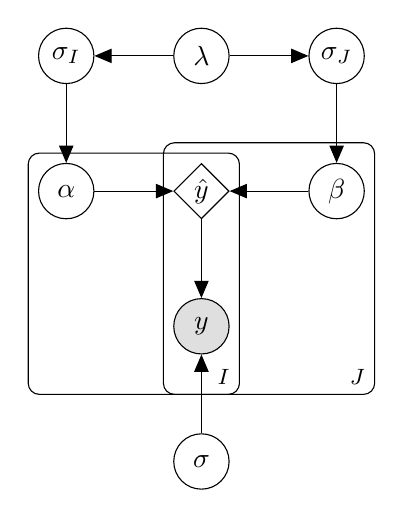
\begin{tikzpicture}

            \node[obs] (y) {$y$};
            \node[det, above=of y] (yhat) {$\hat{y}$};
            \node[latent, left=of yhat] (alpha) {$\alpha$};
            \node[latent, above=of yhat] (lambda) {$\lambda$};
            \node[latent, right=of yhat] (beta) {$\beta$};
            \node[latent, left=of lambda] (sigi) {$\sigma_I$};
            \node[latent, right=of lambda] (sigj) {$\sigma_J$};
            \node[latent, below=of y] (sigma) {$\sigma$};
            
            \edge {sigi} {alpha};
            \edge {sigj} {beta};
            \edge {sigma, yhat} {y};
            \edge {lambda} {sigi};
            \edge {lambda} {sigj};
            \edge {alpha,beta} {yhat};
        
            \plate {I} {(y)(yhat)(alpha)} {$I$};
            \plate {J} {(y)(yhat)(beta)(I.north east)} {$J$};
          
        \end{tikzpicture}}
        \caption{}
    \end{subfigure}
    \hspace{0.1in}
    \begin{subfigure}[b]{0.3\textwidth}

    \begin{minted}{julia1}
m = @model I,J begin
    λ ~ HalfCauchy()
    σI ~ HalfNormal(λ)
    σJ ~ HalfNormal(λ)
     
    α ~ Normal(0, σI) |> iid(I)
    β ~ Normal(0, σJ) |> iid(J)
    yhat = α .+ β'

    σ ~ HalfNormal()
    y ~ For(I,J) do i,j 
            Normal(yhat[i,j], σ)
        end
    end
    \end{minted} 
    \caption{}
    \end{subfigure}

    \caption{A generative model (a), plate diagram (b), and Soss model (c) for a two-way analysis of variance model. Note the specification that $y$ will later be observed is not part of the model, but is instead given at inference time.}
    \label{fig:model}
\end{figure}

\subsection{Joint Distributions}

A Soss model is \emph{function-like}, taking values for its arguments and returning a \emph{joint distribution}. For example, given \jl#m# from Figure~\ref{fig:model}, we can build the joint distribution \jl#d=m(I=2, J=3)#. This supports the usual \jl#rand# and \jl#logpdf# functions, as well as some others provided by Soss described in the following sections. For example,\footnote{This and future outputs are lightly edited for space, for example rounding floating point values.}

\begin{minted}{julia1}
julia> d = m(I=2, J=3); rand(d) # or just rand(m(I=2, J=3))
(I = 2, J = 3, yhat = [-0.52 -1.5 0.0037; -0.81 -1.85 -0.28], σ = 2.5, λ = 1.3, σJ = 0.72, σI = 0.41, 
 β = [-0.54, -1.5, -0.023], α = [0.026, -0.26], y = [-0.45 -2.0 2.2; -3.4 -3.9 2.3])
\end{minted}

\subsection{Inference Primitives}

A given inference algorithm can be expressed in terms of a collection of functions on a model or joint distribution. For example, we often need to evaluate the log-density or its gradient  or draw random samples. In Soss, these \emph{inference primitives} generate model-specific code at execution time.

At this writing, the following inference primitive are available:

\begin{description}  
    \item[\texttt{rand}] draws a random point or sample from a given distribution.
    \item[\texttt{particles}] draws a \emph{systematic sample}, as described in \cite{Douc2005}.
    \item[\texttt{logpdf}] takes a distribution and a point, and returns the log-density at that point.
    \item[\texttt{xform}] takes a distribution and some known data, and returns a bijection from $\mathbb{R}^n$ to the space of unknowns. This is useful for algorithms like Hamiltonian Monte Carlo \cite{Neal2011}.
    \item[\texttt{symlogpdf}] takes a model, and returns a SymPy \cite{10.7717/peerj-cs.103} representation of the log-density, with some additional Julia-based simplifications.
    \item[\texttt{codegen}] calls \jl#symlogpdf#, and uses the result to generate a more efficient version of \jl#logpdf#.
\end{description}

In the above, a \emph{distribution} refers to a joint distribution, while \emph{point} refers to a named tuple in the space space of a distribution.

\todo[inline]{cite MonteCarloMeasurements.jl and TransformVariables.jl}

The set of inference primitives is not fixed, but can be extended by users. New primitives can be added in outside packages, and does not require making changes to the Soss codebase. 

\subsection{Inference}

Together with automatic differentiation, the above inference primitives enable a wide variety of inference algorithms. Rather than building such algorithms specific to Soss, we defer this to external packages. So far, our focus has been Hamiltonian Monte Carlo \cite{Neal2011}, as implemented in \jl#DynamicHMC.jl# \cite{tamas_k_papp_2019_3590018} and \jl#AdvancedHMC.jl# \cite{ge2018t}; Soss has interfaces to these in the {\bf \texttt{dynamicHMC}} and {\bf \texttt{advancedHMC}} functions, respectively.

\subsection{Functions on Models}

Soss includes several functions for querying sets of variables associated with a model. As described above, models are function-like, with the inputs given by {\bf \texttt{arguments}}. In the body of a model every statement declares that some variable is either {\bf \texttt{sampled}} or {\bf \texttt{assigned}}. The sampled and assigned variables together comprise the {\bf \texttt{parameters}}, and all of the above are {\bf \texttt{variables}}. Each of these is a Soss function that takes a model and returns a vector of distinct Julia symbols.

Soss ignores the ordering of statements given by the user, instead working in terms of the DAG ordering. You can access this graph with {\bf \texttt{digraph}}, or use {\bf \texttt{poset}} to get the partial order. Finally, {\bf \texttt{toposort}} returns a topologically-ordered vector of the parameters. Each of these three functions takes a model as input.

Soss represents and manipulates variable dependencies using \jl#SimpleGraphs#, \jl#SimplePosets#, and \jl#SimplePartitions# from \cite{SimpleWorld}.
 

\subsection{Model Transformations}

\begin{description}
    \item[\texttt{Do}] implements Pearl's {\footnotesize\texttt{do}} operator for causal intervention \cite{Pearl1995}.\footnote{Our {\footnotesize\texttt{Do}} operator is capitalized because {\footnotesize\texttt{do}} is a keyword in Julia.}
    \item[\texttt{predictive}] is like \jl#Do#, but only returns the strongly-connected components containing the specified variables. This is useful for sampling from the posterior predictive distribution.
    \item[\texttt{markovBlanket}]  takes a model and a variable, and returns a model representing the Markov blanket at the given variable.
\end{description}

\section{Implementation}

Soss's inference primitives generate code on demand using the \jl#GeneralizedGenerated.jl# library, which introduces a \jl#@gg# macro that works as an extension of Julia's built-in \jl#@generated# macro for \emph{generated functions} \cite{bezanson2012julia}. Similarly to \jl#@generated#, code generated using a \jl#@gg# function cannot depend on the values of its arguments, but only on their types. 

This is problematic, since we clearly need code generation to depend on the model itself. To address this, \jl#GeneralizedGenerated# includes facilities for lifting Julia values to the type level. 

Using this, the type of a Soss model is \jl#Model{A,B,M}#, where 
\begin{itemize}
    \item \jl#A# gives the type of the \emph{arguments} (\jl#A=NamedTuple{T}# for some tuple of symbols \jl#T#),
    \item \jl#B# is a type-level representation of the \emph{body}, and
    \item \jl#M# is a type-level representation of the \emph{module} in which the model was defined.
\end{itemize}

In this, the ``body'' is the \jl#begin...end# following the (possibly empty) arguments of a model. Knowing the module is important in case values from that module are referenced in the model.


\begin{figure}[t]
    \begin{subfigure}[b]{0.48\textwidth}
        \begin{minted}[autogobble]{julia1}
        struct Model{A,B,M} 
            args  :: Vector{Symbol}
            vals  :: NamedTuple
            dists :: NamedTuple
            retn  :: Union{Nothing, Symbol, Expr}
        end

        julia> m.dists
        ( λ = :(HalfCauchy())
        , σI = :(HalfNormal(λ))
        , σJ = :(HalfNormal(λ))
        , α = :(Normal(0, σI) |> iid(I))
        , β = :(Normal(0, σJ) |> iid(J))
        , σ = :(HalfNormal())
        , y = :(For(I, J) do i, j
                Normal(yhat[i, j], σ)
                end))
        \end{minted}

    \end{subfigure}    
    \begin{subfigure}[b]{0.48\textwidth}
        \begin{minted}[autogobble]{julia1}
            julia> m.vals
            (yhat = :(α .+ β'),)

            julia> typeof(m)
            Model{NamedTuple{(:I, :J),T} where T<:Tuple,
                TypeEncoding(begin
                    σ ~ HalfNormal()
                    λ ~ HalfCauchy()
                    σJ ~ HalfNormal(λ)
                    σI ~ HalfNormal(λ)
                    β ~ Normal(0, σJ) |> iid(J)
                    α ~ Normal(0, σI) |> iid(I)
                    yhat = α .+ β'
                    y ~ For(I, J) do i, j
                            Normal(yhat[i, j], σ)
                        end
                end),TypeEncoding(Main)}
        \end{minted}
    \end{subfigure}    
    \caption{The definition of the \texttt{Model} type, and some details of the \texttt{m} model from Figure \ref{fig:model}.}
\end{figure}

The flexibility of code generation in Soss makes it difficult to measure performance. When a performance bottleneck is found, developers or users can ask Soss to generate something different. This design places no a priori constraints on performance.

\todo[inline]{Restructure my writing?}

Besides the purely static code generation via regular macros happening in parsing time, Soss heavily uses a mechanism of "zero-cost" runtime code generation originated by Julia's generated functions \cite{bezanson2012julia}, a.k.a staged functions in the original paper and earlier versions of Julia Programming Language.

The generated functions provide the capability of performing code generation during type inference, generating programs computed by the body of function(a.k.a, generator), once and only once for each combination of argument types.

Further, Julia enables type inference and compiler optimizations equivalent to non-runtime ones in runtime for the callsites of generated functions, hence we gain runtime code generation without losing performance.

To take advantage of this, Soss designs a system to encode sufficient information for generating actual codes, into the types, or objects that can be dispatched like types, which allows the use of generated functions here.

Unfortunately, in current stage, there're some implementation restrictions to Julia's generated functions, and generated functions cannot generate arbitrary Julia codes,
where some advanced programming constructions are missing, such as generators and function-related stuffs like closures(including functions with no free variables), multiple dispatch, etc.

To address this, we introduced the works of easing the restrictions of Julia generated functions,
\todo[inline]{cite GG here?}
which allow us to generate closures from generated functions, and make the programs sufficiently powerful.

Programs that can be generated by Soss are turing complete, as all constructs of Lambda Calculus can be generated.

% \begin{minted}{julia1}
%   abstract type LCTerm end
%   struct Lam{Arg, Body <: LCTerm} <: LCTerm end
%   struct App{Fn<:LCTerm, Arg<:LCTerm} <: LCTerm end
%   struct Var{N} <: LCTerm end
  
%   cg(::Type{Lam{Arg, Term}}) where {Arg, Term} = 
%     :($Arg -> $(cg(Term)))
%   cg(::Type{App{Fn, Arg}}) where {Fn, Arg} = 
%     :($(cg(Fn))($(cg(Arg))))
%   cg(::Type{Var{N}}) where N = N

%   function tolc(expr)
%     @match expr begin
%       :($f($arg)) => App{tolc(f), tolc(arg)}
%       :($x => $y) => Lam{x, tolc(y)}
%       a::Symbol => Var{a}
%     end
%   end
  
%   @gg function lc(::Type{Term}) where Term <: LCTerm
%       cg(Term)
%   end
  
%   macro lc(term)
%     lc(tolc(term))
%   end
  
%   x = Core.Box()
%   y = Core.Box()
%   z = Core.Box()
%   f(x) = (x, z)
%   @assert (@lc x => x)(x) === (@lc y => y)(x)
%   @assert (@lc f => x => f(x))(f)(y) === (y, z)
%   \end{minted} 



\section{Extending Soss}

\section{Related Work}

The idea of code generation and symbolic simplification in an embedded PPL goes back to \emph{Passage} \cite{Scherrer2012}. 

\emph{Hakaru} \cite{narayanan2016probabilistic} takes a more ambitious symbolic approach in a stand-alone PPL, allowing a wider variety of program transformations. 

Soss began with a goal of representing models with continuous, fixed-dimensionality parameter spaces, inspired by \emph{Stan} \cite{stan:2017}.

\emph{Gen} \cite{Cusumano-Towner:2019} was developed independently from Soss, but takes a similar approach (and distinct from most PPLs) in its representation of a model as a function from its arguments to a "trace" (to use Gen's terminology). In both Soss and Gen's static DSL, this trace is a mapping from variable names to values. The similarity of these systems makes interoperability relatively straightforward, as demonstrated in \emph{SossGen} (\url{https://github.com/cscherrer/SossGen.jl}).

\emph{Turing} \cite{ge2018t}

\begin{acks}
We would like to acknowledge...
\end{acks}

\bibliographystyle{acm-reference-format}
\bibliography{ref}

\appendix

\section{Model Syntax}

\begin{figure}[!t]
  \centering
  %\fbox{\rule[-.5cm]{0cm}{\linedwid} \rule[-.5cm]{4cm}{0cm}}
  % using the backnaur package
\begin{bnf*}
  \bnfprod{model}{\bnfts{@model} \bnfsp \bnfpn{args} \bnfsp \bnfts{begin} \bnfsp \bnfpn{statements} \bnfsp \bnfts{end}}\\
  \bnfprod{args}{\bnfes \bnfor \bnfpn{Symbol} \bnfor \bnfpn{Symbol} \bnfts{,} \bnfpn{args}} \\
  \bnfprod{statements}{\bnfpn{statement} \bnfor \bnfpn{statement} \bnfsp \bnftd{Julia Line Sep} \bnfsp \bnfpn{statements} \bnfor \bnfpn{statements} \bnfsp \bnfpn{retn}} \\ 
  \bnfprod{statement}{\bnfpn{assign} \bnfor \bnfpn{sample}} \\
  \bnfprod{assign}{\bnfpn{Symbol} \bnfsp \bnfts{=} \bnfsp \bnfpn{Expr}} \\
  \bnfprod{sample}{\bnfpn{Symbol} \bnfsp \bnfts{\textasciitilde}} \bnfsp \bnfpn{Measure} \\
  \bnfprod{retn}{\bnfts{return} \bnfsp \bnfpn{Expr}} \\
  \bnfprod{Symbol}{\bnftd{Julia Symbol}} \\ 
  \bnfprod{Expr}{\bnftd{Julia Expr}} \\
  \bnfprod{Measure}{\bnftd{Probability measure (see text)}}
\end{bnf*}
  \caption{Backus-Naur Form representation for a user-specified model.}
  \label{fig:bnf}
  \Description{Placeholder figure.}
\end{figure}

\section{Symbolic Simplification}
 
\begin{figure}[t!]
    \centering
    
    \begin{subfigure}[t]{0.4\textwidth}
        \[
    \begin{aligned}
        \ell = 
           &- 3 \log{\left(2 \right)} 
            - 5 \log{\left(\pi \right)} 
            - σ^{2} 
        \\ &- 4 \log{\left(λ \right)} 
            - 2 \log{\left(λ^{2} + 1 \right)} 
            - \frac{σ_I^{2}}{λ^{2}} 
            - \frac{σ_J^{2}}{λ^{2}}
        \\ &+ \sum_{i=1}^{I} \left(- \log{\left(σ_I \right)} - \frac{\log{\pi }}{2} - \frac{\log{2 }}{2}     - \frac{{α}_{i}^{2}}{2 σ_I^{2}}\right) 
        \\ &+ \sum_{j=1}^{J} \left(- \log{\left(σ_J \right)} - \frac{\log{\pi }}{2} - \frac{\log{2 }}{2}     - \frac{{β}_{j}^{2}}{2 σ_J^{2}}\right) 
        \\ &+ \sum_{\substack{1 \leq i \leq I \\ 1 \leq j \leq J}} \left(- \log{\left(σ \right)} - \frac    {\log{\pi }}{2} - \frac{\log{2 }}{2} - \frac{\left({y}_{ij} - {\hat{y}}_{ij}\right)^{2}}{2 σ^{2}    }\right) 
    \end{aligned}
    \]
    \caption{Direct implementation}
    \end{subfigure}
    \hfill
    \begin{subfigure}[t]{0.4\textwidth} 
        \[
    \begin{aligned}
    \ell =
    &- 7.8 - 0.92 I - 0.92 J - 0.92 I J - σ^{2} 
    \\ &- 4 \log{λ } - 2 \log{\left(λ^{2} + 1 \right)} 
        - I J \log{σ } 
    \\ &- I \log{σ_I } - J \log{σ_J } - \frac{σ_I^{2}}{λ^{2}}  - \frac{σ_J^{2}}{λ^{2}}
    \\ &- \frac{1}{2 σ_I^{2}} \sum_{i=1}^{I} {α}_{i}^{2}
        - \frac{1}{2 σ_J^{2}} \sum_{j=1}^{J} {β}_{j}^{2}
    \\ &- \frac{1}{2 σ^{2}} \sum_{\substack{1 \leq i \leq I\\1 \leq j \leq J}} \left({y}_{ij} - {\hat{y}}_{ij}\right)^{2}
    \end{aligned}
\]
    \captionsetup{skip=27pt}
    \caption{After symbolic simplification}
    \end{subfigure}
    \caption{Symbolic log-density of $m$ before (a) and after (b) simplification steps.}
    \label{}
\end{figure}

\begin{figure}[t]
\centering
\begin{subfigure}[t]{0.48\textwidth}
\begin{minted}{julia1}
julia> Soss.sourceRand()(m)
quote
    σ = rand(HalfNormal())
    λ = rand(HalfCauchy())
    σJ = rand(HalfNormal(λ))
    σI = rand(HalfNormal(λ))
    β = rand(iid(J, Normal(0, σJ)))
    α = rand(iid(I, Normal(0, σI)))
    yhat = α .+ β'
    y = rand(For(I, J) do i, j
                Normal(yhat[i, j], σ)
            end)
    (I=I, J=J, yhat=yhat, λ=λ, σI=σI, 
    σJ=σJ, α=α, β=β, σ=σ, y=y) 
end
\end{minted}
\caption{\footnotesize{\texttt{rand}}}
\end{subfigure}
\begin{subfigure}[t]{0.48\textwidth}
\begin{minted}{julia1}
julia> Soss.sourceLogpdf()(m)
quote
    _ℓ = 0.0
    _ℓ += logpdf(HalfNormal(), σ)
    _ℓ += logpdf(HalfCauchy(), λ)
    _ℓ += logpdf(HalfNormal(λ), σJ)
    _ℓ += logpdf(HalfNormal(λ), σI)
    _ℓ += logpdf(Normal(0, σJ) |> iid(J), β)
    _ℓ += logpdf(Normal(0, σI) |> iid(I), α)
    yhat = α .+ β'
    _ℓ += logpdf(For(I, J) do i, j
                Normal(yhat[i, j], σ)
            end, y)
    return _ℓ
end
\end{minted}
\caption{\footnotesize{\texttt{logpdf}}}
\end{subfigure}
\caption{Generated code when calling \footnotesize{\texttt{rand(m)}} and \footnotesize{\texttt{logpdf(m,x)}}.} 
\label{} 
\end{figure}




\section{Extended example }
\todo[inline]{Break this up! This is just a staging area}

\begin{minted}{julia1}
julia> using Revise, Soss, Random

julia> Random.seed!(1);

julia> m = @model I,J begin
           λ ~ HalfCauchy()
           σI ~ HalfNormal(λ)
           σJ ~ HalfNormal(λ)
           α ~ Normal(0, σI) |> iid(I)
           β ~ Normal(0, σJ) |> iid(J)
           yhat = α .+ β'
           σ ~ HalfNormal()
           y ~ For(I,J) do i,j 
                   Normal(yhat[i,j], σ)
               end
       end;

julia> truth = rand(m(I=2,J=3)); pairs(truth);

julia> post = dynamicHMC(m(I=2,J=3), (y=truth.y,));

julia> postpred = predict(m(I=2,J=3), post) |> particles;

julia> postpred.yhat
2×3 Array{Particles{Float64,1000},2}:
 0.241 ± 0.26  0.527 ± 0.3   -0.556 ± 0.38
 0.22 ± 0.26   0.506 ± 0.32  -0.577 ± 0.37

julia> postpred.y
2×3 Array{Particles{Float64,1000},2}:
 0.224 ± 0.58  0.529 ± 0.58  -0.58 ± 0.64
 0.223 ± 0.56  0.483 ± 0.58  -0.58 ± 0.61

julia> m.args
2-element Array{Symbol,1}:
 :I
 :J

julia> pairs(m.vals)
pairs(::NamedTuple) with 1 entry:
  :yhat => :(α .+ β')

julia> pairs(m.dists)
pairs(::NamedTuple) with 7 entries:
  :λ  => :(HalfCauchy())
  :σI => :(HalfNormal(λ))
  :σJ => :(HalfNormal(λ))
  :α  => :(Normal(0, σI) |> iid(I))
  :β  => :(Normal(0, σJ) |> iid(J))
  :σ  => :(HalfNormal())
  :y  => :(For(I, J) do i, j…

\end{minted}

\end{document}
